\pagestyle{fancy}
\chapter{Θεωρία και Μεθοδολογία}
\section{Θεωρία}
Με δεδομένες τις διαστάσεις σε κάτοψη του στοιχείου θεμελίωσης, όπως αυτές αναφέρονται στον (Πίν. \ref{tab:geometry}), θεωρείται πως έχει προηγηθεί επιτυχώς ο έλεγχος της φέρουσας ικανότητας του εδάφους. Κριτήριο στο παρόν στάδιο είναι η αντοχή του ίδιου του πεδίλου. Όλοι οι έλεγχοι αντοχής του πεδίλου γίνονται με υπόθεση γραμμικής κατανομής τάσεων εδάφους ${\sigma}$ κατά τις διευθύνσεις $x$ και $y$. Οι έλεγχοι αυτοί θεωρούν δηλαδή, ότι το πέδιλο μπορεί να αστοχήσει προτού το έδαφος φτάσει τη φέρουσα ικανότητά του.

\section{Μεθοδολογία}
Σε αυτό το σημείο ορίζονται τρία μεγέθη που είναι απαραίτητα για τη συνέχεια. Οι ροπές $M_{x}$ και $M_{y}$ στο κέντρο της βάσης του πεδίλου ισοδυναμούν με δράση της $N_{tot}$ με εκκεντρότητες $e_{x}$ και $e_{y}$ κατά τους άξονες $x$ και $y$ αντίστοιχα.
\begin{equation}
  N_{tot} = N + b_x b_y ({\gamma}_{\sigma\kappa} h + {\gamma}_{\varepsilon\delta}(t - h))\label{eqn:21}
\end{equation}
\begin{equation}
  e_{x} = \dfrac{M_{x}}{N_{tot}}, e_{y} = \dfrac{M_{y}}{N_{tot}}\label{eqn:22}
\end{equation}
\subsection{Διάτμηση}
Ο έλεγχος σε διάτμηση ξεκινά από μία κάθετη διατομή στο οριζόντιο επίπεδο που ορίζει το πέδιλο, σε απόσταση $d$ από την παρειά σύνδεσης πεδίλου - κατακόρυφου στοιχείου. Στη γενική περίπτωση υπάρχουν τέσσερις τέτοιες διατομές (Σχ. \ref{fig:shear}), δύο κάθετες στον άξονα $x$ και δύο στον $y$. Με την παραδοχή μονοαξονικής εκκεντρότητας, ορίζονται οι αποστάσεις των δύο διατομών από τον άξονα $y$, $s_x$ και $s'_x$ και οι αποστάσεις των άλλων δύο διατομών από τον άξονα $x$, $s_y$ και $s'_y$. Από τις δύο κάθετες σε κάθε άξονα διατομές, η μία είναι κρίσιμη (μεγαλύτερη τιμή τέμνουσας), συνεπώς προκύπτουν δύο τέμνουσες σχεδιασμού, μία για κάθε διεύθυνση.

\noindent
Για μονοαξονική εκκεντρότητα $e_x$ και $\dfrac{\abs{e_x}}{b_x} \leq \dfrac{1}{6}$:
\begin{subequations}
\begin{align}
  V_{Ed,x} & = N_{tot}\left(1 + \dfrac{3\abs{e_x}}{b_x}\left(1 + \dfrac{2s_x}{b_x}\right)\right)\left(0.5 - \dfrac{s_x}{b_x}\right) - \left(N_{tot} - N\right)\left(0.5 - \dfrac{s_x}{b_x}\right) \label{eqn:23a} \\[5pt]
  V'_{Ed,x} & = N_{tot}\left(1 - \dfrac{3\abs{e_x}}{b_x}\left(1 - \dfrac{2s'_x}{b_x}\right)\right)\left(0.5 + \dfrac{s'_x}{b_x}\right) - \left(N_{tot} - N\right)\left(0.5 + \dfrac{s'_x}{b_x}\right) \label{eqn:23b}
\end{align}
\end{subequations}
Για μονοαξονική εκκεντρότητα $e_x$ και $\dfrac{\abs{e_x}}{b_x} > \dfrac{1}{6}$:
\begin{subequations}
\begin{align}
  V_{Ed,x} & = \dfrac{4}{9}N_{tot}\dfrac{\left(2.5 - \dfrac{6\abs{e_x}}{b_x} + \dfrac{s_x}{b_x}\right)\left(0.5 - \dfrac{s_x}{b_x}\right)}{\left(1-\dfrac{2\abs{e_x}}{b_x}\right)^2} - \left(N_{tot} - N\right)\left(0.5 - \dfrac{s_x}{b_x}\right) \label{eqn:24a} \\[5pt]
  V'_{Ed,x} & = \dfrac{4}{9}N_{tot}\dfrac{\left(1 - \dfrac{3\abs{e_x}}{b_x} + \dfrac{s'_x}{b_x}\right)^2}{\left(1-\dfrac{2\abs{e_x}}{b_x}\right)^2} - \left(N_{tot} - N\right)\left(0.5 + \dfrac{s'_x}{b_x}\right) \label{eqn:24b}
\end{align}
\end{subequations}
Για μονοαξονική εκκεντρότητα $e_y$ και $\dfrac{\abs{e_y}}{b_y} \leq \dfrac{1}{6}$:
\begin{subequations}
\begin{align}
  V_{Ed,y} & = N_{tot}\left(1 + \dfrac{3\abs{e_y}}{b_y}\left(1 + \dfrac{2s_y}{b_y}\right)\right)\left(0.5 - \dfrac{s_y}{b_y}\right) - \left(N_{tot} - N\right)\left(0.5 - \dfrac{s_y}{b_y}\right) \label{eqn:25a} \\[5pt]
  V'_{Ed,y} & = N_{tot}\left(1 - \dfrac{3\abs{e_y}}{b_y}\left(1 - \dfrac{2s'_y}{b_y}\right)\right)\left(0.5 + \dfrac{s'_y}{b_y}\right) - \left(N_{tot} - N\right)\left(0.5 + \dfrac{s'_y}{b_y}\right) \label{eqn:25b}
\end{align}
\end{subequations}
Για μονοαξονική εκκεντρότητα $e_y$ και $\dfrac{\abs{e_y}}{b_y} > \dfrac{1}{6}$:
\begin{subequations}
\begin{align}
  V_{Ed,y} & = \dfrac{4}{9}N_{tot}\dfrac{\left(2.5 - \dfrac{6\abs{e_y}}{b_y} + \dfrac{s_y}{b_y}\right)\left(0.5 - \dfrac{s_y}{b_y}\right)}{\left(1-\dfrac{2\abs{e_y}}{b_y}\right)^2} - \left(N_{tot} - N\right)\left(0.5 - \dfrac{s_y}{b_y}\right) \label{eqn:26a} \\[5pt]
  V'_{Ed,y} & = \dfrac{4}{9}N_{tot}\dfrac{\left(1 - \dfrac{3\abs{e_y}}{b_y} + \dfrac{s'_y}{b_y}\right)^2}{\left(1-\dfrac{2\abs{e_y}}{b_y}\right)^2} - \left(N_{tot} - N\right)\left(0.5 + \dfrac{s'_y}{b_y}\right) \label{eqn:26b}
\end{align}
\end{subequations}
\noindent
Για διαξονική εκκεντρότητα οι τέμνουσες σχεδιασμού δίνονται πάλι από τις ίδιες σχέσεις με απόλυτη ακρίβεια ή κατά προσέγγιση στην περίπτωση ανάπτυξης αδρανούς περιοχής.

\begin{figure}[H]
  \centering
  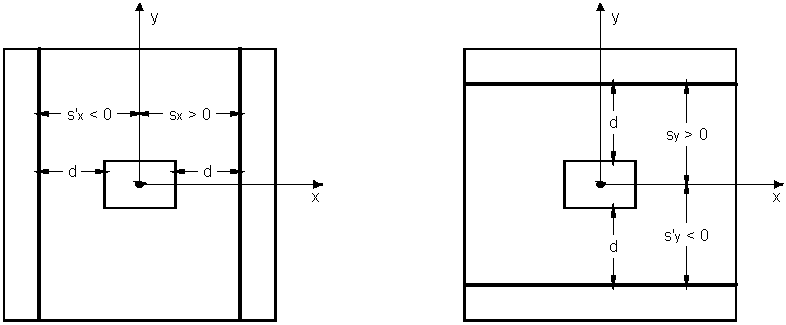
\includegraphics[width=0.8\textwidth,keepaspectratio]{shear}
  \caption{Κρίσιμες διατομές για τον έλεγχο πεδίλου σε διάτμηση}
  \label{fig:shear}
\end{figure}

Οι δύο κρίσιμες τέμνουσες σχεδιασμού συγκρίνονται με την αντοχή σε τέμνουσα ανά διεύθυνση. Ελέγχεται δηλαδή αν:
\begin{subequations}
\begin{align}
  V_{Ed,x} \leq V_{Rd1,x} & = \left(\max\left\{\dfrac{180}{{\gamma}_c}\left(100{\rho}_{1,x}\right)^{1/3}, 35\sqrt{1 + \sqrt{\dfrac{0.2}{d}}}{f_{ck}}^{1/6}\right\}\left(1 + \sqrt{\dfrac{0.2}{d}}\right){f_{ck}}^{1/3}\right){b_y}d\label{eqn:27a}\\[5pt]
  V_{Ed,y} \leq V_{Rd1,y} & = \left(\max\left\{\dfrac{180}{{\gamma}_c}\left(100{\rho}_{1,y}\right)^{1/3}, 35\sqrt{1 + \sqrt{\dfrac{0.2}{d}}}{f_{ck}}^{1/6}\right\}\left(1 + \sqrt{\dfrac{0.2}{d}}\right){f_{ck}}^{1/3}\right){b_x}d\label{eqn:27b}
\end{align}
\end{subequations}
\noindent
Όπου ${\gamma}_c = 1.5$ και ${\rho}_{1,x}$, ${\rho}_{1,y}$ τα γεωμετρικά ποσοστά των ράβδων οπλισμού της κάτω επιφάνειας που διαπερνούν τις κρίσιμες διατομές.

\subsection{Διάτρηση}
Για σχετικά μικρές εκκεντρότητες $e_x$ και $e_y$, πιο κρίσιμος από τον έλεγχο σε διάτμηση είναι συνήθως ο έλεγχος σε διάτρηση. Ως κρίσιμη διατομή σε διάτρηση ορίζεται η κατακόρυφη επιφάνεια που περιβάλλει τη βάση του κατακορύφου στοιχείου σε απόσταση $0 \leq a \leq 2d$ από την περίμετρό του. Η διατρητική τάση αντοχής, αυξάνεται αντιστρόφως ανάλογα της απόστασης $a$ με μέγιστη τιμή $v_{Rd,max}$.
\begin{subequations}
\begin{align}
  v_{Rd,c}\left(a\right) & = \left(\max\left\{\dfrac{0.18}{{\gamma}_c}\left(100{\rho}_1\right)^{1/3}, 0.035\sqrt{1 + \sqrt{\dfrac{0.2}{d}}}{f_{ck}}^{1/6}\right\}\left(1 + \sqrt{\dfrac{0.2}{d}}\right){f_{ck}}^{1/3}\right)\dfrac{2d}{a}\label{eqn:28a}\\[5pt]
  v_{Rd,max} & = 0.3\left(1 - \dfrac{f_{ck}}{250}\right)f_{cd}\label{eqn:28b}
\end{align}
\end{subequations}
\noindent
Ο έλεγχος που πρέπει να γίνει είναι:
\begin{equation}
  maxv_{Ed}\left(a\right) \leq v_{Rd,c}\left(a\right)\label{eqn:29}
\end{equation}
Η μέγιστη δρώσα διατρητική τάση είναι:
\begin{equation}
  maxv_{Ed}\left(a\right) = \beta\left(a\right)\dfrac{V_{Ed,red}\left(a\right)}{u\left(a\right)d}\label{eqn:210}
\end{equation}
Όπου:
\begin{equation}
  V_{Ed,red}\left(a\right) = \left(1-\dfrac{A'}{b_x b_y}\right)\left(R_N - W_f\right) - \dfrac{12A'}{b_x b_y}\left(\dfrac{a_x e_x}{{b_x}^2} + \dfrac{a_y e_y}{{b_y}^2}\right)R_N\label{eqn:211}
\end{equation}
\begin{equation}
  A' = \pi a^2 + c_x c_y + 2a\left(c_x + c_y\right)\label{eqn:212}
\end{equation}
\begin{equation}
  u \left(a\right) = 2\left(\pi a + c_x + c_y\right)\label{eqn:213}
\end{equation}
Ο συντελεστής $\beta\left(a\right)$ δίνει την αύξηση της δρώσας διατρητικής τάσης ως προς τη μέση δρώσα λόγω εκκεντροτήτων:
\begin{equation}
  e_{x,red}\left(a\right) = \dfrac{M_{Edx,red}\left(a\right)}{V_{Ed,red}\left(a\right)} ,e_{y,red}\left(a\right) = \dfrac{M_{Edy,red}\left(a\right)}{V_{Ed,red}\left(a\right)}\label{eqn:214}
\end{equation}
Η δρώσα μειωμένη ροπή είναι:
\begin{subequations}
\begin{align}
  M_{Edx,red}\left(a\right) & = e_x R_N - \dfrac{A'}{b_x b_y}a_x\left(R_N - W_f\right) - \dfrac{12R_N}{b_x b_y}\left(\dfrac{\left(I_x ' + {a_x}^2 A'\right)e_x}{{b_x}^2} + \dfrac{a_x a_y A' e_y}{{b_y}^2}\right)\label{eqn:215a}\\[5pt]
  M_{Edy,red}\left(a\right) & = e_y R_N - \dfrac{A'}{b_x b_y}a_y\left(R_N - W_f\right) - \dfrac{12R_N}{b_x b_y}\left(\dfrac{\left(I_y ' + {a_y}^2 A'\right)e_y}{{b_y}^2} + \dfrac{a_x a_y A' e_x}{{b_x}^2}\right)\label{eqn:215b}
\end{align}
\end{subequations}
Όπου:
\begin{subequations}
\begin{align}
  W_f & = b_x b_y h {\gamma}_{\sigma\kappa} + \left(b_x b_y - c_x c_y \right)\left(t - h\right){\gamma}_{\varepsilon\delta}\label{eqn:216a}\\[5pt]
  I_x ' & = \dfrac{\pi a^2 \left({c_x}^2 + a^2\right)}{4} + \dfrac{a{c_x}^3}{6} + \dfrac{{c_y} \left(2a + c_x\right)^3}{12}\label{eqn:216b}\\[5pt]
  I_y ' & = \dfrac{\pi a^2 \left({c_y}^2 + a^2\right)}{4} + \dfrac{a{c_y}^3}{6} + \dfrac{{c_x} \left(2a + c_y\right)^3}{12}\label{eqn:216c}
\end{align}
\end{subequations}

\begin{itemize}
  \item Αν $e_{x,red}\left(a\right) > 0$ και $e_{y,red}\left(a\right) = 0$ :
  \begin{equation}
  \beta\left(a\right) = 1 + k e_{x,red}\left(a\right)\dfrac{u\left(a\right)}{W_x\left(a\right)}\label{eqn:217}
  \end{equation}
  \begin{equation}
    W_x\left(a\right) = \dfrac{c_x ^2}{2} + c_x c_y + 2 a c_y + \pi a c_x + 4 a^2\label{eqn:218}
  \end{equation}
    \begin{itemize}
      \item $c_x / c_y \leq 0.5 \rightarrow k = 0.45$, $c_x / c_y = 1.0 \rightarrow k = 0.60$
      \item $c_x / c_y = 2.0 \rightarrow k = 0.70$, $c_x / c_y \geq 3.0 \rightarrow k = 0.80$
    \end{itemize}
  \item Αν $e_{x,red}\left(a\right) = 0$ και $e_{y,red}\left(a\right) > 0$ :
  \begin{equation}
  \beta\left(a\right) = 1 + k e_{y,red}\left(a\right)\dfrac{u\left(a\right)}{W_y\left(a\right)}\label{eqn:219}
  \end{equation}
  \begin{equation}
    W_y\left(a\right) = \dfrac{c_y ^2}{2} + c_x c_y + 2 a c_x + \pi a c_y + 4 a^2\label{eqn:220}
  \end{equation}  
    \begin{itemize}
      \item $c_y / c_x \leq 0.5 \rightarrow k = 0.45$, $c_y / c_x = 1.0 \rightarrow k = 0.60$
      \item $c_y / c_x = 2.0 \rightarrow k = 0.70$, $c_y / c_x \geq 3.0 \rightarrow k = 0.80$
    \end{itemize}
  \item Αν $e_{x,red}\left(a\right) > 0$ και $e_{y,red}\left(a\right) > 0$ :
  \begin{equation}
    \beta\left(a\right) = 1 + 1.8 \sqrt{\left(\dfrac{e_{x,red}\left(a\right)}{c_y + 2 a}\right)^2 + \left(\dfrac{e_{y,red}\left(a\right)}{c_x + 2 a}\right)^2}\label{eqn:221}
  \end{equation}
\end{itemize}

\subsection{Διαστασιολόγηση σε κάμψη}
Το πέδιλο κατά την κάμψη του λειτουργεί σαν ένας ανεστραμμένος διπλός πρόβολος και στις δύο διευθύνσεις $x$ και $y$, με εφελκυσμό στην κάτω επιφάνεια, όπου και τοποθείται εσχάρα οπλισμού με συνολικό εμβαδόν $A_sx$ και $A_sy$ ανά διεύθυνση. Κρίσιμες σε κάμψη διατομές είναι οι παράλληλες στους άξονες $x$ και $y$ κατακόρυφες διατομές του πεδίλου, οι οποίες εφάπτονται της περιμέτρου του υποστυλώματος.\\
Για μονοαξονική εκκεντρότητα $e_x$ και $\dfrac{\abs{e_x}}{b_x} \leq \dfrac{1}{6}$:
\begin{subequations}
\begin{align}
  M_{Ed,x} & = N_{tot}b_x\left(0.5 + \dfrac{2\abs{e_x}}{b_x}\left(1 + \dfrac{s_x}{b_x}\right)\right)\left(0.5 - \dfrac{s_x}{b_x}\right)^2 - 0.5 \left(N_{tot} - N\right)b_x\left(0.5 - \dfrac{s_x}{b_x}\right)^2 \label{eqn:222a}\\[5pt]
  M'_{Ed,x} & = N_{tot}b_x\left(0.5 - \dfrac{2\abs{e_x}}{b_x}\left(1 - \dfrac{s'_x}{b_x}\right)\right)\left(0.5 + \dfrac{s'_x}{b_x}\right)^2 - 0.5 \left(N_{tot} - N\right)b_x\left(0.5 + \dfrac{s'_x}{b_x}\right)^2 \label{eqn:222b}
\end{align}
\end{subequations}
Για μονοαξονική εκκεντρότητα $e_x$ και $\dfrac{\abs{e_x}}{b_x} > \dfrac{1}{6}$:
\begin{subequations}
\begin{align}
  M_{Ed,x} & = \dfrac{4}{27}N_{tot}b_x\dfrac{\left(4 - \dfrac{9\abs{e_x}}{b_x} + \dfrac{s_x}{b_x}\right)\left(0.5 - \dfrac{s_x}{b_x}\right)^2}{\left(1-\dfrac{2\abs{e_x}}{b_x}\right)^2} - 0.5\left(N_{tot} - N\right)b_x\left(0.5 - \dfrac{s_x}{b_x}\right)^2 \label{eqn:223a}\\[5pt]
  M'_{Ed,x} & = \dfrac{4}{27}N_{tot}b_x\dfrac{\left(1 - \dfrac{3\abs{e_x}}{b_x} + \dfrac{s'_x}{b_x}\right)^3}{\left(1-\dfrac{2\abs{e_x}}{b_x}\right)^2} - 0.5\left(N_{tot} - N\right)b_x\left(0.5 + \dfrac{s'_x}{b_x}\right)^2 \label{eqn:223b}
\end{align}
\end{subequations}
Για μονοαξονική εκκεντρότητα $e_y$ και $\dfrac{\abs{e_y}}{b_y} \leq \dfrac{1}{6}$:
\begin{subequations}
\begin{align}
  M_{Ed,y} & = N_{tot}b_y\left(0.5 + \dfrac{2\abs{e_y}}{b_y}\left(1 + \dfrac{s_y}{b_y}\right)\right)\left(0.5 - \dfrac{s_y}{b_y}\right)^2 - 0.5 \left(N_{tot} - N\right)b_y\left(0.5 - \dfrac{s_y}{b_y}\right)^2 \label{eqn:224a}\\[5pt]
  M'_{Ed,y} & = N_{tot}b_y\left(0.5 - \dfrac{2\abs{e_y}}{b_y}\left(1 - \dfrac{s'_y}{b_y}\right)\right)\left(0.5 + \dfrac{s'_y}{b_y}\right)^2 - 0.5 \left(N_{tot} - N\right)b_y\left(0.5 + \dfrac{s'_y}{b_y}\right)^2 \label{eqn:224b}
\end{align}
\end{subequations}
Για μονοαξονική εκκεντρότητα $e_y$ και $\dfrac{\abs{e_y}}{b_y} > \dfrac{1}{6}$:
\begin{subequations}
\begin{align}
  M_{Ed,y} & = \dfrac{4}{27}N_{tot}b_y\dfrac{\left(4 - \dfrac{9\abs{e_y}}{b_y} + \dfrac{s_y}{b_y}\right)\left(0.5 - \dfrac{s_y}{b_y}\right)^2}{\left(1-\dfrac{2\abs{e_y}}{b_y}\right)^2} - 0.5\left(N_{tot} - N\right)b_y\left(0.5 - \dfrac{s_y}{b_y}\right)^2 \label{eqn:225a}\\[5pt]
  M'_{Ed,y} & = \dfrac{4}{27}N_{tot}b_y\dfrac{\left(1 - \dfrac{3\abs{e_y}}{b_y} + \dfrac{s'_y}{b_y}\right)^3}{\left(1-\dfrac{2\abs{e_y}}{b_y}\right)^2} - 0.5\left(N_{tot} - N\right)b_y\left(0.5 + \dfrac{s'_y}{b_y}\right)^2 \label{eqn:225b}
\end{align}
\end{subequations}
Για διαξονική εκκεντρότητα οι τέμνουσες σχεδιασμού δίνονται πάλι από τις ίδιες σχέσεις με απόλυτη ακρίβεια ή κατά προσέγγιση στην περίπτωση ανάπτυξης αδρανούς περιοχής.